\documentclass[10pt,letterpaper,english]{beamer}

\usepackage{ragged2e}
\justifying

\usetheme{default}
\setbeamertemplate{navigation symbols}{\textcolor{blue}{\insertframenumber ~/ \inserttotalframenumber}}

\usepackage{xstring}
\usepackage{pgfpages}
\makeatletter
\IfSubStr{\@classoptionslist}{handout}
  {\pgfpagesuselayout{2 on 1}[letterpaper,border shrink=5mm]}
  {}
\makeatother

\usepackage{amsmath,amssymb,amsthm}
\usepackage{stmaryrd}
\usepackage{enumerate}
\usepackage{stfloats}
\usepackage{bbm}
\usepackage{pdfpages}
\usepackage{framed}
\usepackage{tabularx}
\usepackage[normalem]{ulem}

\usepackage{tikz,pgf,pgfplots}
\usepackage{algorithm,algorithmic}
\usepgflibrary{shapes}
\usetikzlibrary{%
  arrows,%
  arrows.meta,
  shapes.misc,% wg. rounded rectangle
  shapes.arrows,%
  shapes,%
  calc,%
  chains,%
  matrix,%
  positioning,% wg. " of "
  scopes,%
  decorations.pathmorphing,% /pgf/decoration/random steps | erste Graphik
  shadows,%
  backgrounds,%
  fit,%
  petri,%
  quotes
}

%\pgfplotsset{compat=1.12}

%\usetheme{Frankfurt}
%\usecolortheme{ldpc}
\useinnertheme{rounded}
\usecolortheme{whale}
\usecolortheme{orchid}


\newcommand{\ul}[1]{\underline{#1}}
\renewcommand{\Pr}{\mathbb{P}}

\newcommand{\getpdfpages}[2]{\begingroup
  \setbeamercolor{background canvas}{bg=}
  \addtocounter{framenumber}{1}
  \includepdf[pages={#1},%
  pagecommand={%
    \expandafter\def\expandafter\insertshorttitle\expandafter{%
      \insertshorttitle\hfill\insertframenumber\,/\,\inserttotalframenumber}}%
  ]{#2}
  \endgroup}

\newcommand{\backupbegin}{
   \newcounter{finalframe}
   \setcounter{finalframe}{\value{framenumber}}
}
\newcommand{\backupend}{
   \setcounter{framenumber}{\value{finalframe}}
}

 \setbeamercolor{bibliography entry author}{fg=black}
 \setbeamercolor{bibliography entry title}{fg=black}
 \setbeamercolor{bibliography entry location}{fg=black}
 \setbeamercolor{bibliography entry note}{fg=black}
 
 \setbeamerfont{bibliography item}{size=\footnotesize}
 \setbeamerfont{bibliography entry author}{size=\footnotesize}
 \setbeamerfont{bibliography entry title}{size=\footnotesize}
 \setbeamerfont{bibliography entry location}{size=\footnotesize}
 \setbeamerfont{bibliography entry note}{size=\footnotesize}
 \setbeamertemplate{bibliography item}{\insertbiblabel}
 
\newlength\tikzwidth
\newlength\tikzheight

\def\checkmark{\tikz\fill[scale=0.4](0,.35) -- (.25,0) -- (1,.7) -- (.25,.15) -- cycle;}
\def\greencheck{{\color{green}\checkmark}}
\def\scalecheck{\resizebox{\widthof{\checkmark}*\ratio{\widthof{x}}{\widthof{\normalsize x}}}{!}{\checkmark}}
\def\xmark{\tikz [x=1.4ex,y=1.4ex,line width=.2ex, red] \draw (0,0) -- (1,1) (0,1) -- (1,0);}
\def\redx{{\color{red}\xmark}}

\renewcommand{\footnotesep}{-2pt}

\newif\ifslow
\slowtrue

\newcommand{\mc}[1]{\mathcal{#1}}
\newcommand{\mbb}[1]{\mathbb{#1}}
%\newcommand{\expt}{\mbb{E}}
%\newcommand{\dd}{\mathrm{d}}
\newcommand{\Interior}[1]{\ensuremath{{#1}^{\circ}}}
\newcommand{\Closure}[1]{\ensuremath{\overline{#1}}}
\newcommand{\Complement}[1]{\ensuremath{{#1}^{c}}}

\newcommand{\Expect}{\ensuremath{\mathrm{E}}}
\newcommand{\vecnot}{\underline}
\newcommand{\RealNumbers}{\ensuremath{\mathbb{R}}}
\newcommand{\RationalNumbers}{\mathbb{Q}}
\newcommand{\ComplexNumbers}{\mathbb{C}}
\newcommand{\Real}{\mathrm{Re}}
\newcommand{\Span}{\mathrm{span}}
\newcommand{\Rank}{\mathrm{rank}}
\newcommand{\Nullity}{\mathrm{nullity}}
\newcommand{\Trace}{\mathrm{tr}}
\newcommand{\Diag}{\mathrm{diag}}
\newcommand{\dd}{\mathrm{d}}
\DeclareMathOperator*{\esssup}{ess\,sup}

% Use < , > inner product
\newcommand{\inner}[2]{{\left\langle #1 \mskip2mu , #2 \right\rangle}}
\newcommand{\tinner}[2]{{\langle #1 \mskip1mu , #2 \rangle}}

% Use < | > inner product
%\newcommand{\inner}[2]{{\left\langle #1 \mskip2mu \middle| \mskip2mu #2 \right\rangle}}
%\newcommand{\tinner}[2]{{\langle #1 \mskip1mu | \mskip1mu  #2 \rangle}}




\begin{document}

\ifslow

\title{ECE 586: Vector Space Methods \\ Chapter 4: Representation and Approximation}
\author{Henry D. Pfister \\ Duke University}
\date{November 4th--18th, 2019}
\maketitle

\begin{frame}{4.1: Best Approximation}

Let $W$ be a subspace of a Banach space $V$ and, for any $\vecnot{v} \in V$, consider finding a vector $\vecnot{w} \in W$ such that $\left\| \vecnot{v} - \vecnot{w} \right\|$ is as small as possible.
\begin{definition}<1->
The vector $\vecnot{w} \in W$ is a \textcolor{blue}{best approximation} of $\vecnot{v} \in V$ by vectors in $W$ if
\begin{equation*}
\left\| \vecnot{v} - \vecnot{w} \right\| \leq \left\| \vecnot{v} - \vecnot{w}' \right\|
\end{equation*}
for all $\vecnot{w}' \in W$.
\end{definition}

\begin{example}<2->
If $W$ is spanned by the vectors $\vecnot{w}_1, \ldots, \vecnot{w}_n \in V$, then we can write
\begin{equation*}
\vecnot{v} = \vecnot{w} + \vecnot{e} = s_1 \vecnot{w}_1 + \cdots + s_n \vecnot{w}_n + \vecnot{e},
\end{equation*}
where $\vecnot{e} = \vecnot{v}-\vecnot{w}$ is the approximation error.
\end{example}
\end{frame}

\begin{frame}{Vector Projection Revisited}

Let $\vecnot{u},\vecnot{v}$ be vectors in an inner-product space $V$ with inner product $\tinner{ \cdot }{ \cdot }$.

\begin{lemma}<1->
If $\tinner{ \vecnot{w} }{ \vecnot{v} } = 0$, then $\| \vecnot{w} \!+\! \vecnot{v} \|^2 = \| \vecnot{w} \|^2 \!+\! 2\, \text{Re} \{ \tinner{ \vecnot{w} }{ \vecnot{v} }  \} \!+\! \| \vecnot{v} \|^2 = \| \vecnot{w} \|^2 \!+\! \| \vecnot{v} \|^2$.
\end{lemma}

\begin{definition}[Vector Projection]<1->
The \textcolor{blue}{projection} of $\vecnot{w}$ onto $\vecnot{v}$ is defined to be \\[-3mm]
\begin{tabular}{>{\centering}m{2in} m{2in}}
$ \vecnot{u} = \displaystyle\frac{\inner{ \vecnot{w} }{ \vecnot{v} }}{\|\vecnot{v}\|^2} \vecnot{v} $ &
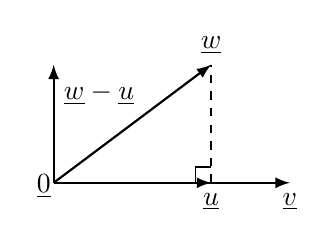
\begin{tikzpicture}[scale=0.5]
  \coordinate (v1) at (0,0);
  \coordinate (v2) at (4,3);
  \coordinate (v3) at (6,0);
  \coordinate (v4) at (4,0);
  \coordinate (v5) at (0,3);
  \path[draw] (3.6,0) -- (3.6,0.4) -- (4,0.4);
  \node (v0) at (-0.25,-0.1) {$\vecnot{0}$};
  \draw[-latex,thick] (v1) -- node[at end,above] {$\vecnot{w}$} (v2);
  \draw[-latex,thick] (v1) -- node[at end,below] {$\vecnot{v}$} (v3);
  \draw[-latex,thick] (v1) -- node[at end, below] {$\vecnot{u}$} (v4);
  \draw[thick,dashed] (v4) --  (v2);
  \draw[-latex,thick] (v1) -- node[right,near end] {$\vecnot{w}-\vecnot{u}$} (v5);
\end{tikzpicture}
\end{tabular}
\vspace{-1,5mm}
\end{definition}


\begin{lemma}
Let $\vecnot{u}$ be the projection of $\vecnot{w}$ onto $\vecnot{v}$.
If $\tinner{ \vecnot{w} }{ \vecnot{v} } \neq 0$, then $\| \vecnot{w} - \vecnot{u} \| < \| \vecnot{w} \|$.
\end{lemma}
\begin{proof}
$\tinner{ \vecnot{w} - \vecnot{u} }{ \vecnot{u} } = 0$ implies $\| \vecnot{w} \|^2 = \| (\vecnot{w}-\vecnot{u}) + \vecnot{u} \|^2 = \| \vecnot{w} -\vecnot{u} \|^2 + \| \vecnot{u} \|^2$.
\end{proof}

\end{frame}

\begin{frame}{4.1: Orthogonal Projection}

In an arbitrary Banach space, finding a best approximation can be hard.

\vspace{2mm}

But, if the norm $\| \cdot \|$ corresponds to the induced norm of a Hilbert space, then \textcolor{blue}{orthogonal projection} greatly simplifies the problem.

\begin{theorem}[Subspace Projection] Suppose $W$ is a subspace of a Hilbert space $V$ and $\vecnot{v} \in V$.
Then,
\begin{enumerate}
\item The vector $\vecnot{w} \in W$ is a best approximation of $\vecnot{v} \in V$ by vectors in $W$ if and only if $\vecnot{v} - \vecnot{w}$ is orthogonal to every vector in $W$.
\item If a best approximation of $\vecnot{v} \in V$ by vectors in $W$ exists, it is unique.
\item If $W$ is a closed subspace with a countable orthogonal basis $\vecnot{w}_1, \vecnot{w}_2, \ldots$, then the best approximation of $\vecnot{v}$ by vectors in $W$ is \vspace{-1.5mm}
\begin{equation*}
\vecnot{w} = \sum_{i=1}^\infty \frac{ \inner{ \vecnot{v} }{ \vecnot{w}_i } }{ \left\| \vecnot{w}_i \right\|^2 } \vecnot{w}_i . \vspace{-1mm}
\end{equation*}
Note: the implied linear mapping $E\colon V \to W$ defined by $E(\vecnot{v}) = \vecnot{w}$ is called the \textcolor{blue}{orthogonal projection} of $V$ onto $W$.
\end{enumerate}
\end{theorem}

Proof on whiteboard.

\end{frame}

\iffalse
\begin{frame}{Orthogonal Projection}

\begin{definition}
Whenever the vector $\vecnot{w}$ in the best approximation theorem exists, it is called the \textcolor{blue}{orthogonal projection} of $\vecnot{v}$ onto $W$.
\end{definition}

\begin{definition}
If every vector in $V$ has an orthogonal projection onto $W$, then the mapping $E \colon V \rightarrow W$, which assigns to each vector in $V$ its orthogonal projection onto $W$, is called the orthogonal projection of $V$ onto $W$.
\end{definition}

\end{frame}
\fi

\begin{frame}{4.1.1: Projections Without Orthogonality (1)}

\begin{definition}
A function $F \colon X \rightarrow Y$ with $Y \subseteq X$ is \textcolor{blue}{idempotent} if $F(F(x))=F(x)$.  When $F$ is a linear transformation, this reduces to $F^2 = F \cdot F = F$.
\end{definition}

\begin{definition}
Let $V$ be a vector space and $T \colon V \rightarrow V$ be a linear transformation.
If $T$ is idempotent, then $T$ is called a \textcolor{blue}{projection} because $T\vecnot{v} = \vecnot{v}$ if $\vecnot{v} \in \mathcal{R}(T)$.
\end{definition}

\begin{example}
The idempotent matrix $A$ is a projection onto the first two coordinates. \vspace{-2mm}
\begin{equation*}
A = \begin{bmatrix}
1 & 0 & 1 \\
0 & 1 & 1 \\
0 & 0 & 0
\end{bmatrix}
\end{equation*}
\end{example}

\end{frame}

\begin{frame}{4.1.1: Projections Without Orthogonality (2)}

\begin{theorem}
Let $V$ be a vector space and $T \colon V \rightarrow V$ be a projection operator.
Then, the range $\mathcal{R}(T)$ and the $\mathcal{N}(T)$ are disjoint subspaces of $V$.
\end{theorem}

\begin{proof}
For a non-zero $\vecnot{v} \in \mathcal{R}(T)$, there is a non-zero $\vecnot{w} \in V$ such that $\vecnot{v} = T\vecnot{w}$.  Thus, $T\vecnot{v} = T^2  \vecnot{w} = T \vecnot{w} = \vecnot{v} \neq \vecnot{0}$.  But, if $\vecnot{v} \in \mathcal{N}(T)$ was also true, then one would get the contradiction $T\vecnot{v} = \vecnot{0}$.
\end{proof}

\begin{example}<2->
Consider the linear transform $T \colon V \rightarrow V$ defined by $T = I - P$, where $P$ is a projection.
It is easy to verify that $T$ is a projection operator because \vspace{-2mm}
\[ T^2 = (I-P)(I-P) = I - P- P + P^2 = I-P = T .\]
In fact, $T$ is a projection onto $\mathcal{R}(T) = \mathcal{N}(P)$ because $P \vecnot{v} = \vecnot{0}$ (i.e., $\vecnot{v} \in \mathcal{N}(P)$) if and only if  $(I-P)\vecnot{v} = \vecnot{v}$ (i.e., $\vecnot{v} \in \mathcal{R}(T)$).
\end{example}

\end{frame}

\begin{frame}{4.1.1: Orthogonal Projection Operators}

\begin{definition}<1->
Let $V$ be an inner-product space and $P \colon V \rightarrow V$ be a projection operator.
If $\mathcal{R}(P) \bot \mathcal{N}(P)$, then $P$ is called an \textcolor{blue}{orthogonal projection} .
\end{definition}

\begin{example}<1->
Let $V$ be an inner-product space and $P \colon V \rightarrow V$ be an orthogonal projection.
Then, $\vecnot{v} = P \vecnot{v} + (I-P) \vecnot{v}$ gives an orthogonal decomposition of $\vecnot{v}$ because $P \vecnot{v} \in \mathcal{R}(P)$, $(I-P) \vecnot{v} \in \mathcal{N}(P)$, and $\mathcal{R}(P) \bot \mathcal{N}(P)$.
\end{example}

\begin{theorem}<2->
For $V=F^n$ with standard inner product, $P$ is an orthogonal projection matrix if it is idempotent and Hermitian (i.e. $P^2=P$ and $P^H = P$).
\end{theorem}
\begin{proof}<3->
Since $\mathcal{R}(P) = \{ P\vecnot{u} | \vecnot{u}\in V \}$ and $\mathcal{N}(P) = \{ \vecnot{v}\in V | P\vecnot{v}=\vecnot{0} \}$, the general condition is $\tinner{ P\vecnot{u} }{ (I-P)\vecnot{v} } =0$ for all $\vecnot{u},\vecnot{v}\in V$.
Simplifying this gives \vspace{-2mm}
\[ \vecnot{v}^H (I-P)^H P \vecnot{u} = \vecnot{v}^H (P - P^H P) \vecnot{u} = \vecnot{v}^H (P - P^2) \vecnot{u} = 0.  \qedhere\]
\end{proof}

\end{frame}

\newcommand*{\vertbar}{\rule[-1ex]{0.5pt}{2.5ex}}

\begin{frame}{4.1.1: Orthogonal Projection onto an Orthonormal Set}

Let $V = \ComplexNumbers^n$ be the standard $n$-dimensional complex Hilbert space and $U \in \ComplexNumbers^{n\times m}$ be a matrix with orthonormal columns $\vecnot{u}_1,\ldots,\vecnot{u}_m$:

\[ U = \begin{bmatrix} \vertbar & \vertbar & & \vertbar \\ \vecnot{u}_1 & \vecnot{u}_2 & \cdots & \vecnot{u}_m \\ \vertbar & \vertbar & & \vertbar \end{bmatrix} \]

\vspace{4mm}

Then, the best approximation of $\vecnot{v}\in V$ by vectors in $\mathcal{R}(U)$, given by
\begin{equation*}
\vecnot{w} = \sum_{i=1}^m \frac{ \inner{ \vecnot{v} }{ \vecnot{u}_i } }{ \left\| \vecnot{u}_i \right\|^2 } \vecnot{u}_i,
\end{equation*}
can also be written as
\[ {\color{blue}\vecnot{w} = U U^H \vecnot{v}} = \sum_{i=1}^m \vecnot{u}_i (\vecnot{u}_i^H \vecnot{v}). \]

\end{frame}


\begin{frame}{4.2: Normal Equations}

Let $W$ be a subspace of a Hilbert space $V$ that is spanned by the linearly independent (but not orthogonal) set of vectors  $\vecnot{w}_1, \ldots, \vecnot{w}_n \in V$.

\vspace{2mm}

The projection theorem shows that $\hat{\vecnot{v}} \in W$ is the best approximation of $\vecnot{v} \in V$ if and only if $(\vecnot{v} - \hat{\vecnot{v}}) \bot \vecnot{w}_j$ for $j=1,\ldots,n$.
This implies that
\begin{equation*}
\inner{ \vecnot{v} - \hat{\vecnot{v}} }{ \vecnot{w}_j }
= \inner{ \vecnot{v} - \sum_{i=1}^n s_i \vecnot{w}_i }{ \vecnot{w}_j }
= 0
\end{equation*}
or, equivalently, the \textcolor{blue}{normal equations}
\begin{equation*}
\sum_{i=1}^n s_i \inner{ \vecnot{w}_i }{ \vecnot{w}_j }
= \inner{ \vecnot{v} }{ \vecnot{w}_j }.
\end{equation*}

The gives a system of $n$ linear equations in $n$ unknowns defined by
\begin{equation*}
\underbrace{\left[ \begin{array}{cccc}
\inner{ \vecnot{w}_1 }{ \vecnot{w}_1 }
& \inner{ \vecnot{w}_2 }{ \vecnot{w}_1 } & \cdots
& \inner{ \vecnot{w}_n }{ \vecnot{w}_1 } \\
\inner{ \vecnot{w}_1 }{ \vecnot{w}_2 }
& \inner{ \vecnot{w}_2 }{ \vecnot{w}_2 } & \cdots
& \inner{ \vecnot{w}_n }{ \vecnot{w}_2 } \\
\vdots & \vdots & \ddots & \vdots \\
\inner{ \vecnot{w}_1 }{ \vecnot{w}_n }
& \inner{ \vecnot{w}_2 }{ \vecnot{w}_n } & \cdots
& \inner{ \vecnot{w}_n }{ \vecnot{w}_n }
\end{array} \right]}_G
\underbrace{\left[ \begin{array}{c}
s_1 \\ s_2 \\ \vdots \\ s_n \end{array} \right]}_\vecnot{s}
= \underbrace{\left[ \begin{array}{c}
\inner{ \vecnot{v} }{ \vecnot{w}_1 } \\
\inner{ \vecnot{v} }{ \vecnot{w}_2 } \\ \vdots \\
\inner{ \vecnot{v} }{ \vecnot{w}_n } \end{array} \right]}_\vecnot{t} .
\end{equation*}

\end{frame}

\begin{frame}{4.2: The Gramian}

\begin{definition}<1->
For $\vecnot{w}_1,\ldots,\vecnot{w}_n$, the $n \times n$ \textcolor{blue}{Gramian matrix} is defined to be \vspace{-1.5mm}
\begin{equation*}
G = \left[ \begin{array}{cccc}
\inner{ \vecnot{w}_1 }{ \vecnot{w}_1 }
& \inner{ \vecnot{w}_2 }{ \vecnot{w}_1 } & \cdots
& \inner{ \vecnot{w}_n }{ \vecnot{w}_1 } \\
\inner{ \vecnot{w}_1 }{ \vecnot{w}_2 }
& \inner{ \vecnot{w}_2 }{ \vecnot{w}_2 } & \cdots
& \inner{ \vecnot{w}_n }{ \vecnot{w}_2 } \\
\vdots & \vdots & \ddots & \vdots \\
\inner{ \vecnot{w}_1 }{ \vecnot{w}_n }
& \inner{ \vecnot{w}_2 }{ \vecnot{w}_n } & \cdots
& \inner{ \vecnot{w}_n }{ \vecnot{w}_n }
\end{array} \right] \vspace{-1mm}
\end{equation*}
Since $g_{ij} = \inner{ \vecnot{w}_j }{ \vecnot{w}_i }$, we see $G$ is Hermitian symmetric (i.e. $G^H = G$).
\end{definition}

\begin{definition}<2->
A matrix $M\in F^{n \times n}$ is \textcolor{blue}{positive-semidefinite} if $M=M^H$ and $\vecnot{v}^H M \vecnot{v} \geq 0$ for all $\vecnot{v} \in F^n - \left\{ \vecnot{0} \right\}$.
If the inequality is strict, then it is \textcolor{blue}{positive-definite}.
\end{definition}


\begin{theorem}<2->
A Gramian matrix $G$ is always positive-semidefinite.
It is positive-definite if and only if the vectors $\vecnot{w}_1, \ldots, \vecnot{w}_n$ is linearly independent.
\end{theorem}

\visible<2->{Proof on whiteboard.}

\end{frame}

\begin{frame}{4.3: Least-Squares Solution of a Linear System}

\visible<1->{%
For $V = F^m$, let $A \in F^{m \times n}$ be a matrix whose $i$-th column is $\vecnot{w}_i \in V$.
Then, a vector $\hat{\vecnot{v}} \in W = \text{colspace}(A)$ can be written as
\[ \hat{\vecnot{v}} = A \vecnot{s} = \sum_{i=1}^n s_i \vecnot{w}_i. \]

Also, the best approximation of $\vecnot{v}$ by vectors in $W$ is found by solving
\[ \min_{\hat{\vecnot{v}}\in W} \| \vecnot{v} - \hat{ \vecnot{v}} \| = \min_\vecnot{s} \| \vecnot{v} - A \vecnot{s} \| . \]
}

\vspace{-2mm}

\visible<2->{%
For the induced norm, any solution must satisfy the normal equations
\[ \inner{ \vecnot{v} - \hat{\vecnot{v}} }{ \vecnot{w}_j }
= \inner{ \vecnot{v} - A \vecnot{s} }{ \vecnot{w}_j }
= 0, \quad j \in [n]. \]
}

\vspace{-4mm}

\visible<3->{%
For the standard inner product, these equations can be expressed as
\begin{equation*}
\vecnot{0} = \left[ \begin{array}{c} \vecnot{w}_1^H \\ \vdots \\ \vecnot{w}_n^H \end{array} \right] \left( \vecnot{v} - A \vecnot{s} \right) = A^H \vecnot{v} - A^H A \vecnot{s} = \vecnot{t} - G \vecnot{s},
\end{equation*}
where \textcolor{blue}{$G = A^H A$ is the Gramian} and \textcolor{blue}{$\vecnot{t}$ is the cross-correlation vector.}}
\end{frame}

\begin{frame}{4.3.2: Pseudo-Inverse and Projection}

\visible<1->{%
When the vectors $\vecnot{w}_1, \ldots, \vecnot{w}_n$ are linearly independent, the Gramian matrix is positive definite and hence invertible.
Thus, the optimal solution for the least-squares problem is given by
\begin{equation*}
\vecnot{s} = G^{-1} \vecnot{t} = \left( A^H A \right)^{-1} A^H \vecnot{v},
\end{equation*}
where the matrix \textcolor{blue}{$\left( A^H A \right)^{-1} A^H$ is the pseudoinverse} of $A$ in this case.}

\vspace{7mm}

\visible<2->{%
Using this, the best approximation of $\vecnot{v} \in V$ by vectors in $W$ is equal to
\begin{equation*}
\hat{\vecnot{v}} = A \vecnot{s} = A \left( A^H A \right)^{-1} A^H \vecnot{v} .
\end{equation*}
The matrix \textcolor{blue}{$P = A \left( A^H A \right)^{-1} A^H$ is the projection matrix} for the range of $A$.
It defines an orthogonal projection onto the range of $A$ (i.e., the subspace spanned by the columns of $A$).}

\end{frame}

\begin{frame}{4.3.3: Weighted Least-Squares Solution of a Linear System}

For the standard Euclidean norm $\| \vecnot{v} \|_E = \sqrt{\vecnot{v}^H \vecnot{v}}$ and any invertible $B$, consider the weighted least-squares problem
\[ \min_{\hat{\vecnot{v}}\in W} \| B(\vecnot{v} - \hat{ \vecnot{v}}) \|_E = \min_\vecnot{s} \| B( \vecnot{v} - A \vecnot{s}) \|_E \]
But, $\| B \vecnot{v} \|_E$ equals the induced norm $\| \vecnot{v} \|$ for the weighted inner product
\[ \inner{ \vecnot{u} }{ \vecnot{v} }  \triangleq \vecnot{v}^H B^H B \vecnot{u}. \]

For the weighted inner product, the normal equations look the same
\[ \inner{ \vecnot{v} - \hat{\vecnot{v}} }{ \vecnot{w}_j }
= \inner{ \vecnot{v} - A \vecnot{s} }{ \vecnot{w}_j }
= 0, \quad j \in [n]. \]
but they solve a different problem and they reduce to
\begin{equation*}
\vecnot{0} = \left[ \begin{array}{c} \vecnot{w}_1^H \\ \vdots \\ \vecnot{w}_n^H \end{array} \right] B^H B \left( \vecnot{v} - A \vecnot{s} \right) = A^H B^H B \vecnot{v} - A^H B^H B A \vecnot{s}
\end{equation*}

\end{frame}

\iffalse
\begin{frame}{4.3.4: Expression for Minimum Approximation Error}

Let $\hat{\vecnot{v}} \in W$ be the best approximation of $\vecnot{v}$ by vectors in $W$. Then,
\begin{equation*}
\vecnot{v} = \hat{\vecnot{v}} + \vecnot{e},
\end{equation*}
where $\vecnot{e} \in W^{\bot}$ is the minimum achievable error.
The squared norm of the minimum error is given implicitly by
\begin{equation*}
\left\| \vecnot{v} \right\|^2
= \left\| \hat{\vecnot{v}} + \vecnot{e} \right\|^2
= \inner{ \hat{\vecnot{v}} + \vecnot{e} }{ \hat{\vecnot{v}} + \vecnot{e} }
= \inner{ \hat{\vecnot{v}} }{ \hat{\vecnot{v}} }
+ \inner{ \vecnot{e} }{ \vecnot{e} }
= \left\| \hat{\vecnot{v}} \right\|^2 + \left\| \vecnot{e} \right\|^2 .
\end{equation*}
For the weighted problem, let $H=B^H B$ and write
\begin{equation*}
\begin{split}
\left\| \vecnot{e} \right\|^2
&= \left\| \vecnot{v} \right\|^2
- \left\| \hat{\vecnot{v}} \right\|^2
= \vecnot{v}^H H \vecnot{v} - \hat{\vecnot{v}}^H H \hat{\vecnot{v}} \\
&= \vecnot{v}^H H \vecnot{v} - \vecnot{s}^H A^H H A \vecnot{s} \\
&= \vecnot{v}^H H \vecnot{v}
- \vecnot{v}^H H A \left( A^H H A \right)^{-1} A^H H \vecnot{v} \\
&= \vecnot{v}^H
\left( H -  H A \left( A^H H A \right)^{-1} A^H H \right)
\vecnot{v}.
\end{split}
\end{equation*}
\end{frame}
\fi

\begin{frame}{4.4.2: Linear Minimum Mean-Squared Error Estimation}

Let $Y, X_1, \ldots, X_n$ be zero-mean random variables.
Linear minimum mean-squared error (LMMSE) estimation finds $s_1, \ldots, s_n$ such that
\[ \hat{Y} = s_1 X_1 + \cdots + s_n X_n \]
minimizes the mean squared-error $\Expect[|Y-\hat{Y}|^2]$.
Using the inner product
\begin{equation*}
\inner{ X }{ Y } = \Expect \left[ X \overline{Y} \right],
\end{equation*}
the normal equations for the LMMSE estimate $\hat{Y}$ are $G \vecnot{s} = \vecnot{t}$, where
\begin{equation*}
G = \left[ \begin{array}{cccc}
\Expect \left[ X_1 \overline{X}_1 \right]
& \Expect \left[ X_2 \overline{X}_1 \right] & \cdots
& \Expect \left[ X_n \overline{X}_1 \right] \\
\Expect \left[ X_1 \overline{X}_2 \right]
& \Expect \left[ X_2 \overline{X}_2 \right] & \cdots
& \Expect \left[ X_n \overline{X}_2 \right] \\
\vdots & \vdots & \ddots & \vdots \\
\Expect \left[ X_1 \overline{X}_n \right]
& \Expect \left[ X_2 \overline{X}_n \right] & \cdots
& \Expect \left[ X_n \overline{X}_n \right] \\
\end{array} \right], \quad \vecnot{t} = \left[ \begin{array}{c}
\Expect \left[ Y \overline{X}_1 \right] \\
\Expect \left[ Y \overline{X}_2 \right] \\ \vdots \\
\Expect \left[ Y \overline{X}_n \right] \end{array} \right].
\end{equation*}

If the matrix $G$ is invertible, the minimum mean-squared error is given by
\begin{equation*}
\left\| Y - \hat{Y} \right\|^2 = \Expect \left[ Y \overline{Y} \right]
- \left[ \hat{Y} \overline{\hat{Y}} \right] = \Expect \left[ Y \overline{Y} \right] - \vecnot{t}^H G^{-1} \vecnot{t} .
\end{equation*}

\end{frame}

\begin{frame}{4.5.1: Dual Approximation and Minimum-Norm Solutions}

An underdetermined system of linear equations has an infinite number of solutions.
It often makes sense to prefer the \textcolor{blue}{minimum-norm solution}.

\vspace{3mm}

Let $V$ be a Hilbert space and $\vecnot{w}_1 ,\vecnot{w}_2 , \ldots, \vecnot{w}_n$ be a basis for subspace $W$.
For any $\vecnot{v} \in V$, the best approximation of $\vecnot{v}$ in $W$ can be found by solving
\begin{equation} \label{eqn:DualNormalEquations}
\left[ \begin{array}{cccc}
\inner{ \vecnot{w}_1 }{ \vecnot{w}_1 }
& \inner{ \vecnot{w}_2 }{ \vecnot{w}_1 } & \cdots
& \inner{ \vecnot{w}_n }{ \vecnot{w}_1 } \\
\inner{ \vecnot{w}_1 }{ \vecnot{w}_2 }
& \inner{ \vecnot{w}_2 }{ \vecnot{w}_2 } & \cdots
& \inner{ \vecnot{w}_n }{ \vecnot{w}_2 } \\
\vdots & \vdots & \ddots & \vdots \\
\inner{ \vecnot{w}_1 }{ \vecnot{w}_n }
& \inner{ \vecnot{w}_2 }{ \vecnot{w}_n } & \cdots
& \inner{ \vecnot{w}_n }{ \vecnot{w}_n }
\end{array} \right]
\left[ \begin{array}{c}
s_1 \\ s_2 \\ \vdots \\ s_n \end{array} \right]
= \left[ \begin{array}{c}
\inner{ \vecnot{v} }{ \vecnot{w}_1 } \\
\inner{ \vecnot{v} }{ \vecnot{w}_2 } \\ \vdots \\
\inner{ \vecnot{v} }{ \vecnot{w}_n } \end{array} \right] .
\end{equation}

\begin{theorem}
Let $V$ be a Hilbert space and $\vecnot{w}_1 ,\vecnot{w}_2 , \ldots, \vecnot{w}_n$ be a basis for $W\subseteq V$.
The \textcolor{blue}{dual approximation} problem is to find the minimum-norm vector $\vecnot{w}\in V$ satisfying $\inner{ \vecnot{w} }{ \vecnot{w}_i } = c_i$ for $i=1,\ldots,n$.
Then, the solution $\vecnot{w}$ satisfies \vspace{-1.5mm}
\[ \vecnot{w} = \sum_{i=1}^n s_i \vecnot{w}_i \in W, \vspace{-1.5mm} \]
where $s_1,s_2,\ldots,s_n$ can be found by solving \eqref{eqn:DualNormalEquations} with $\inner{ \vecnot{v} }{ \vecnot{w}_i } = c_i$.
\end{theorem}

\end{frame}

\begin{frame}{4.5.2: Minimum-Norm Solutions}

\visible<1->{%
For $A \in \ComplexNumbers^{m\times n}$ with $m<n$ and $\vecnot{v} \in \ComplexNumbers^m$, consider the underdetermined linear system $A \vecnot{s} = \vecnot{v}$.
Then, the dual approximation theorem can be applied to solve the minimum-norm problem
\[ \min_{\vecnot{s} : A\vecnot{s} = \vecnot{v}} \| \vecnot{s} \| . \]
}

\vspace{1mm}

\visible<2->{%
To see this as a dual approximation, we can rewrite the constraint $A \vecnot{s} = \vecnot{v}$ as $B^H \vecnot{s} = \vecnot{v}$ where $B = A^H$.
Then, the theorem concludes that the minimum-norm solution lies in  the column space of $B=A^H$.}

\vspace{4mm}

\visible<3->{%
Using $\vecnot{s} \in \mathcal{R}(A^H)$, there is a $\vecnot{t}$ such that $\hat{\vecnot{s}} = A^H \vecnot{t}$ and the constraint gives $A (A^H \vecnot{t}) = \vecnot{v}$.
If the rows of $A$ are linearly independent, then the columns of $B=A^H$ are linearly independent and $(B^H B)^{-1} = (A A^H)^{-1}$ exists.

\vspace{4mm}

Thus, the solution $\hat{\vecnot{s}}$ can be obtained in closed form and is given by \vspace{-1mm}
\[ \color{blue} \hat{\vecnot{s}} = A^H \left( A A^H \right)^{-1} \vecnot{v}. \]
}

\end{frame}

\begin{frame}{6.5: The Four Fundamental Subspaces}

Consider a linear transform mapping $\RealNumbers^n \to \RealNumbers^m$ represented by $A\in \RealNumbers^{m\times n}$

\begin{itemize}
\setlength\itemsep{1mm}

\item<1-> The four fundamental subspaces are: $\mathcal{R}(A)$, $\mathcal{N}(A)$, $\mathcal{R}(A^T)$, $\mathcal{N}(A^T)$

\item<1-> Recall $A^T \in \RealNumbers^{n\times m}$ maps $\RealNumbers^m \to \RealNumbers^n$ and \textcolor{blue}{$\mathcal{R}(A^T)$ is the row space of $A$}

\vspace{3mm}

\item<2-> Notice that $\vecnot{x} \in \RealNumbers^n$ is in the \textcolor{blue}{null space of $A$} \emph{if and only if} \vspace{-1mm}
\[ A \vecnot{x} = \begin{bmatrix} -- \text{row 1} -- \\ -- \text{row 2} -- \\ \vdots \\ -- \text{row m} -- \end{bmatrix} \vecnot{x} = \begin{bmatrix} 0 \\ 0 \\ \vdots \\ 0 \end{bmatrix} \]
\emph{if and only if} \textcolor{blue}{all rows orthogonal to $\vecnot{x}$} under standard inner product

\vspace{3mm}

\item<3-> Thus, the \textcolor{blue}{null space of $A$} is \textcolor{red}{orthogonal} to the \textcolor{blue}{column space of $A^T$} 

\item<4-> Symmetry: \textcolor{blue}{null space of $A^T$} is \textcolor{red}{orthogonal} to the \textcolor{blue}{column space of $A$} 

\vspace{2mm}

\item<5-> In our notation, this means that $\mathcal{N}(A) \bot \mathcal{R}(A^T)$ and $\mathcal{N}(A^T) \bot \mathcal{R}(A)$

\end{itemize}
\end{frame}

\begin{frame}{6.5: The Four Fundamental Subspaces: Linear Equations}

\hspace*{-1mm}
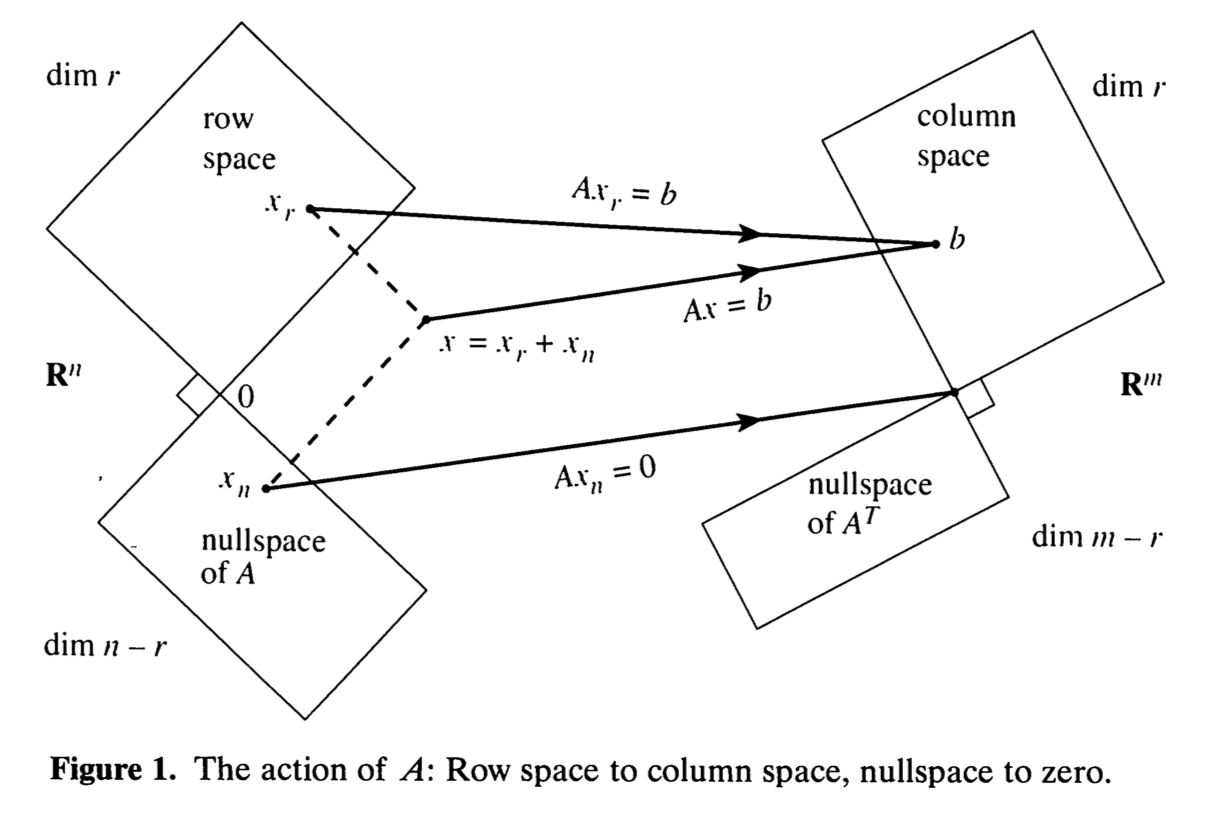
\includegraphics[width=108mm]{strang_fig1.png}

\vspace{-3mm}
$r \triangleq \dim(\mathcal{R}(A))$ implies \textcolor{blue}{$\dim ( \mathcal{N}(A)) = n\!-\!r$} and \textcolor{blue}{$\dim ( \mathcal{N}(A^T)) = m\!-\!r$}

\let\thefootnote\relax\footnotetext{\hspace*{-4mm} {\tiny Figure from ``The Fundamental Theorem of Linear Algebra'' by Gilbert Strang, The American Mathematical Monthly, Nov. 1993 }}

\end{frame}

\begin{frame}{6.5: The Four Fundamental Subspaces: Least Squares}

\hspace*{-4mm}
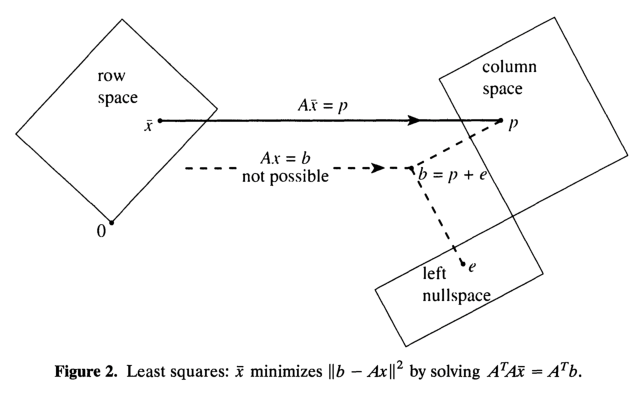
\includegraphics[width=114mm]{strang_fig2}

Observe $A^T A \colon \RealNumbers^n \to \RealNumbers^n$ is invertible if non-singular (i.e., if $n=r$)

\let\thefootnote\relax\footnotetext{\hspace*{-4mm} {\tiny Figure from ``The Fundamental Theorem of Linear Algebra'' by Gilbert Strang, The American Mathematical Monthly, Nov. 1993 }}

\end{frame}

\begin{frame}{Interlude: Alternative for Linear Systems}

A ``Theorem of the Alternative'' asserts that exactly one of two logical statements is true. The following is a famous example.

\begin{theorem}
For a matrix $A \in \mathbb{R}^{m\times n}$ and a vector $\vecnot{b}\in \mathbb{R}^m$, exactly one of the following statements is true:
\begin{itemize}
\item There exists an $\vecnot{x}\in \mathbb{R}^n$ such that $A\vecnot{x} = \vecnot{b}$
\item There exists a $\vecnot{y} \in \mathbb{R}^m$ such that $A^T \vecnot{y} = \vecnot{0}$ and $\vecnot{y}^T \vecnot{b} \neq 0$.
\end{itemize} 
\end{theorem}

\begin{proof}<2->
\begin{itemize}
\item In the first case, $\vecnot{b} \in \mathcal{R}(A)$ and the four fundamental subspaces imply that $\vecnot{y}^T \vecnot{b} = 0$ (i.e., $\vecnot{y} \perp \vecnot{b}$) if $A^T \vecnot{y} = \vecnot{0}$ (i.e., $\vecnot{y}\in \mathcal{N}(A^T)$).
\item In the second case, $\vecnot{y} \in \mathcal{N}(A^T)$ implies $\vecnot{y} \perp \mathcal{R}(A)$.
So, $\vecnot{y}^T \vecnot{b} \neq 0$ implies $\vecnot{b} \notin \mathcal{R}(A)$. \qedhere
\end{itemize}
\end{proof}

%\visible<3->{Choosing $m=n$, one can also add ``for all $\vecnot{b}\in W$'' to the first statement and ``there exists $\vecnot{b}\in W$'' to the second statement.}

\end{frame}


\begin{frame}{8: Eigenvalue Decomposition}

\begin{definition}<1->
Let $V$ be a vector space over $F$ and let $T\colon V \to V$ be a linear operator.
An \textcolor{blue}{eigenvalue} of $T$ is a scalar $\lambda \in F$ such that there exists a non-zero vector $\vecnot{v} \in V$ with $T \vecnot{v} = \lambda \vecnot{v}$.
Any vector $\vecnot{v}$ such that $T \vecnot{v} = \lambda \vecnot{v}$ is called an \textcolor{blue}{eigenvector} of $T$ associated with the eigenvalue value $\lambda$.
\end{definition}

\begin{definition}<2->
The square matrix $B$ is \textcolor{blue}{diagonalizable} if there is an invertible matrix $S$ (whose columns are eigenvectors) such that $S^{-1} B S = \Lambda$ is diagonal.
\end{definition}

%\begin{lemma}
%Let $A$ be a Hermitian matrix (i.e., $A^H = A$).
%Then, all eigenvalues of $A$ are real and eigenvectors with different eigenvalues are orthogonal.
%\end{lemma}

%\begin{proof}
%First, we notice that $A = A^H$ implies $\vecnot{v}^H A \vecnot{v}$ is real because \vspace{-1mm}
%\[ \overline{s} = \left( \vecnot{v}^H A \vecnot{v} \right)^H = \vecnot{v}^H A^H \vecnot{v} = \vecnot{v}^H A \vecnot{v} = s. \vspace{-1mm} \]
%If $A \vecnot{v} = \lambda_1 \vecnot{v}$, left multiplication by $\vecnot{v}^H$ shows $\vecnot{v}^H A \vecnot{v} = \lambda_1 \vecnot{v}^H \vecnot{v} = \lambda_1 \| \vecnot{v} \|$.
%Thus, $\lambda_1$ is real.
%Next, assume that $A \vecnot{w} = \lambda_2 \vecnot{w}$ and $\lambda_2 \neq \lambda_1$ so that \vspace{-1mm}
%\[ \lambda_1 \lambda_2 \vecnot{w}^H \vecnot{v} = \vecnot{w}^H A^H A \vecnot{v} = \vecnot{w} A^2 \vecnot{v} = \lambda_1^2 \vecnot{w}^H \vecnot{v}. \]
%We also assume, without loss of generality, that $\lambda_1 \neq 0$.
%Therefore, if $\lambda_2 \neq \lambda_1$, then $\vecnot{w}^H \vecnot{v} = 0$ and the eigenvectors are orthogonal.
%\end{proof}

\begin{theorem}<3->
Any Hermitian matrix $B$ can be diagonalized by a unitary matrix $U$ so that $U^H B U = \Lambda$ is a real-valued diagonal matrix.
\end{theorem}

\vspace{2mm}

\visible<4->{
Matrices $A^H A$ and $A A^H$ are always Hermitian and positive semidefinite}

\end{frame}


\begin{frame}{9: Singular Value Decomposition (SVD)}

Idea is to find orthonormal bases for $\RealNumbers^n$ and $\RealNumbers^m$ in which $A$ is diagonal

\begin{itemize}
\setlength\itemsep{3mm}

\item<1-> Let $\vecnot{v}_1, \ldots, \vecnot{v}_r$ be orthonormal eigenvectors of $A^H A$ with positive eigenvalues $\sigma_1^2,\ldots,\sigma_r^2$.
Then, \[\|A \vecnot{v}_i\| ^2 = \vecnot{v}_i^H (A^H A \vecnot{v}_i) =  \vecnot{v}_i^H (\sigma_i^2\vecnot{v}_i) = \sigma_i^2 \]

\item<2-> This implies that $\|A \vecnot{v}_i\| = \sigma_i$.
So $\vecnot{u}_i = \frac{1}{\sigma_i} A\vecnot{v}_i$ has $\| \vecnot{u}_i \| \!=\! 1$ and \vspace{-1mm}
\begin{align*}
A A^H \vecnot{u}_i &= \frac{1}{\sigma_i} A A^H A \vecnot{v}_i = \frac{1}{\sigma_i} \sigma_i^2 A \vecnot{v}_i = \vecnot{u}_i
\\
\vecnot{u}_j^H \vecnot{u}_i &= \left(\frac{1}{\sigma_j} A \vecnot{v}_j \right)^H \left(\frac{1}{\sigma_i} A \vecnot{v}_i \right) =\frac{1}{\sigma_i \sigma_j} \vecnot{v}_j^H (A^H A) \vecnot{v}_i = \delta_{i,j}  \vspace{-1mm}
\end{align*}


\item<3-> For $U_1 = [\vecnot{u}_1,\ldots,\vecnot{u}_r]
$ and $V_1 = [\vecnot{v}_1,\ldots,\vecnot{v}_r]$, this gives $A V_1 = U_1 \Sigma_1$ where $\Sigma_1$ is a $r \times r$ diagonal matrix with diagonal entries $\sigma_1,\ldots,\sigma_r$

\item<4-> Solving for $A$ gives the \textcolor{blue}{compact SVD} \vspace{-1mm} \[ \color{blue} A = U_1 \Sigma V_1^H, \vspace{-1mm}\]
where the \textcolor{blue}{columns of $U_1, V_1$ are orthonormal bases for $\mathcal{R}(A), \mathcal{R}(A^H)$}

\end{itemize}


\end{frame}

\begin{frame}{9: The Four Fundamental Subspaces: Orthogonal Bases}

\vspace{-1mm}
\hspace*{-1mm}
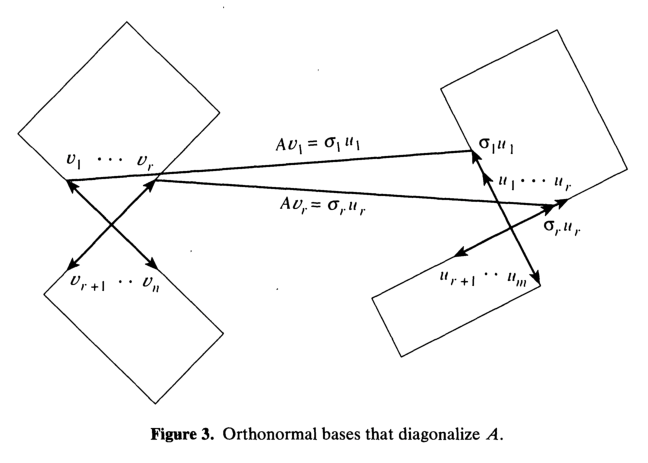
\includegraphics[width=102mm]{strang_fig3}

\vspace{-3mm}
For $V = [\vecnot{v}_1,\ldots,\vecnot{v}_n]
$ and $U = [\vecnot{u}_1,\ldots,\vecnot{u}_m]$, $A V = U \Sigma$ where $\Sigma \in \RealNumbers^{m \times n}$ has diagonal $\sigma_1,\ldots,\sigma_r$.  Thus, $A = U \Sigma V^H$.


\let\thefootnote\relax\footnotetext{\hspace*{-4mm} {\tiny Figure from ``The Fundamental Theorem of Linear Algebra'' by Gilbert Strang, The American Mathematical Monthly, Nov. 1993 }}

\end{frame}

\begin{frame}{6.5: The Four Fundamental Subspaces: Pseudo-Inverse}

\hspace*{-4mm}
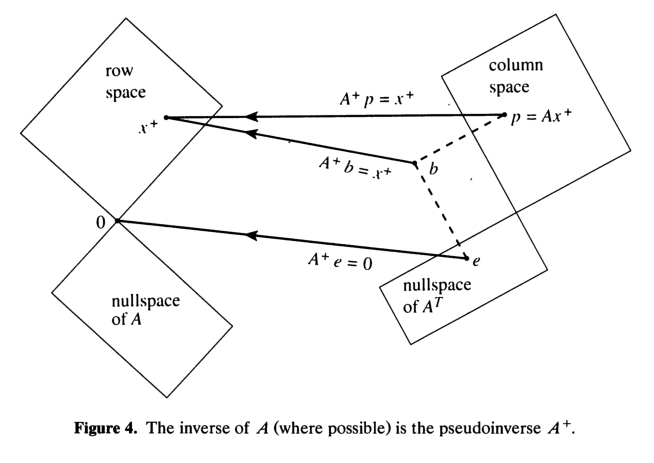
\includegraphics[width=114mm]{strang_fig4}

\let\thefootnote\relax\footnotetext{\hspace*{-4mm} {\tiny Figure from ``The Fundamental Theorem of Linear Algebra'' by Gilbert Strang, The American Mathematical Monthly, Nov. 1993 }}

\end{frame}

\begin{frame}{9.2: Singular Value Decomposition Example}

\visible<1->{%
Consider the matrix 
\[ A = \left[ \begin{array}{cc}
1 & 1 \\
5 & -1 \\
-1 & 5 
\end{array} \right]. \]}

\visible<2->{%
An eigenvalue decomposition of $A^H A$ is given by
\[ \!\!\!\!\!\!\!\!\!\!\!\! A^H A \!=\! \left[ \begin{array}{cc}
27 & -9 \\
-9 & 27
\end{array} \right]
\!=\! V \Lambda V^H
\!=\! \left( \frac{1}{\sqrt{2}}\left[ \begin{array}{cc}
-1 & 1 \\
1 & 1 
\end{array} \right] \right)
\left[ \begin{array}{cc}
36 & 0 \\
0 & 18
\end{array} \right]
\left( \frac{1}{\sqrt{2}} \left[ \begin{array}{cc}
-1 & 1 \\
1 & 1 
\end{array} \right] \right)
\]}

\visible<3->{%
This implies $\Sigma_1 = \Lambda^{1/2}$ and $V_1 = V$.
Thus, we find $U_1 = A V_1 \Sigma_1^{-1}$ with
\[ U_1 = \left[ \begin{array}{cc}
1 & 1 \\
5 & -1 \\
-1 & 5 
\end{array} \right]
\left( \frac{1}{\sqrt{2}} \left[ \begin{array}{cc}
-1 & 1 \\
1 & 1
\end{array} \right] \right)
\left[ \begin{array}{cc}
\frac{1}{\sqrt{36}} & 0 \\
0 & \frac{1}{\sqrt{18}}
\end{array} \right]
= \left[ \begin{array}{cc}
0 & \frac{1}{3} \\
\frac{1}{\sqrt{2}} & \frac{2}{3}  \\
-\frac{1}{\sqrt{2}} & \frac{2}{3} 
\end{array} \right] \]}

\vspace{-1mm}

\visible<4->{%
Putting this all together, we have the compressed SVD
\[ A = U_1 \Sigma_1 V_1^H 
= \left[ \begin{array}{cc}
0 & \frac{1}{3} \\
\frac{1}{\sqrt{2}} & \frac{2}{3}  \\
-\frac{1}{\sqrt{2}} & \frac{2}{3} 
\end{array} \right]
\left[ \begin{array}{cc}
\sqrt{36} & 0 \\
0 & \sqrt{18}
\end{array} \right]
\left( \frac{1}{\sqrt{2}} \left[ \begin{array}{cc}
-1 & 1 \\
1 & 1 
\end{array} \right] \right). \]}

\end{frame}

\begin{frame}{Moore--Penrose Pseudo Inverse}

For a matrix $A \in \ComplexNumbers^{m\times n}$, the matrix $A^+ \in \ComplexNumbers^{n\times m}$ is the pseudo-inverse iff:
\begin{enumerate}
\item $A A^+ A = A$ (implies $A A^+$ is idempotent)
\item $A^+ A A^+ = A^+$ (implies $A^+ A$ is idempotent)
\item $(A A^+)^H = A A^+$ (implies $A A^+$ is Hermitian)
\item $(A^+ A)^H = A^+ A$ (implies $A^+ A$ is Hermitian)
\end{enumerate}

\begin{lemma}
From the compact SVD $A = U_1 \Sigma_1 V_1^H$, one finds that $A^+ = V_1
\Sigma_1^{-1} U_1^H$.
\end{lemma}

\begin{proof}<2->
\begin{enumerate}
\item $A A^+ A = U_1 {\color{blue}(\Sigma_1 V_1^H  V_1
\Sigma_1^{-1} U_1^H  U_1)} \Sigma_1 V_1^H = A $
\item $A^+ A A^+ =  V_1
{\color{blue}(\Sigma_1^{-1} U_1^H U_1 \Sigma_1 V_1^H  V_1)}
\Sigma_1^{-1} U_1^H  = A^+$
\item $(A A^+)^H = \big(U_1 {\color{blue}(\Sigma_1 V_1^H V_1
\Sigma_1^{-1})} U_1^H \big)^H  = {U_1 U_1^H} = A A^+$
\item $(A^+ A)^H = \big(V_1 {\color{blue}(\Sigma_1^{-1} U_1^H U_1
\Sigma_1)} V_1^H \big)^H  = {V_1 V_1^H} = A^+ A$ \qedhere
\end{enumerate}
\end{proof}

\visible<2->{Thus, $A A^+$ and $A^+ A$ are projection matrices onto $\mathcal{R}(A)$ and $\mathcal{R}(A^H)$.}

\end{frame}

\backupbegin

%\begin{frame}
%\frametitle{Backup Slides}
%\begin{itemize}
%\item Slide numbers not included in denominator!
%\end{itemize}
%\end{frame}

%\begin{frame}[allowframebreaks]
%\frametitle{References}
%\bibliographystyle{alpha}
%\footnotesize
%\bibliography{IEEEabrv,WCLabrv,WCLbib,WCLnewbib}
%\end{frame}

\backupend

\end{document}
